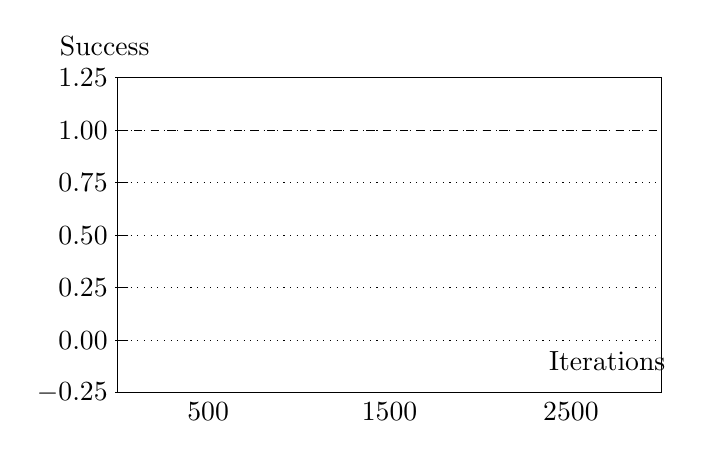
\begin{tikzpicture}[x=0.0023cm,y=2.6666cm]
    % Draw the axes and grid lines
    \draw[-] (0,-0.25) -- (0,1.25) -- (3000,1.25) -- (3000,-0.25) -- cycle; 
    \draw[-,thin, dotted, ystep=0.25, xstep=3000] (0,-0.25) grid (3000,1.25);
%    \foreach \x in {500, 1500, 2500}  \draw [-,xshift=0,yshift=-0.25](\x,4pt) -- (\x,-1pt);
    \foreach \y in {-0.25,0.00,0.25,0.50,0.75,1.00,1.25}  \draw [-,yshift=0](4pt,\y) -- (-1pt,\y);
    \foreach \x/\xtext in {500/500, 1500/1500, 2500/2500} \node at (\x,-0.25) [below] {$\xtext$};
    \foreach \y/\ytext in {-0.25,0.00,0.25,0.50,0.75,1.00,1.25}  \node at (0,\y) [left] {$\ytext$};
    \node at (-70,1.4) {Success};
    \node at (2700,-0.1) {Iterations};
    \draw[-] plot[mark=x,mark size=4,mark options={color=black}] 
			file {data/test05v3gmt.CC.tikzdata};
    \draw[-,thin,densely dashed,gray] plot[mark=x,mark size=4,mark options={color=gray}] 
			file {data/test05v3gmt.CP.tikzdata};
%    \draw[-] plot[mark=diamond,mark size=4,mark options={color=black}] 
%			file {data/test05v3gmt.SC.tikzdata};
    \draw[-] plot[mark=o,mark size=2,mark options={color=black}] 
			file {data/test05v3gmt.SP.tikzdata};
    % Also draw the expected convergence: 0.9^8 actions=0.43046
    \draw[dashed,-,yshift=0](0,1.0) -- (3000,1.0);

\end{tikzpicture}
